\documentclass[10pt,twocolumn,letterpaper]{article}

\usepackage[utf8]{inputenc}
\usepackage{cvpr}
\usepackage{times}
\usepackage{epsfig}
\usepackage{graphicx}
\usepackage{amsmath,amsfonts,amssymb,amsthm}
\usepackage{color}
\usepackage{caption}
\usepackage{subcaption}
\usepackage{xspace}
\usepackage{xcolor}
\usepackage{array}
\usepackage{cite}
\usepackage{tabularx}
\usepackage{multirow}
\usepackage[pagebackref=true,breaklinks=true,colorlinks,bookmarks=false]{hyperref}

\cvprfinalcopy
\def\cvprPaperID{1708}
\def\httilde{\mbox{\tt\raisebox{-.5ex}{\symbol{126}}}}
%\ifcvprfinal\pagestyle{empty}\fi

\newcommand{\Perp}{\perp\!\!\! \perp}
\newcommand{\bK}{\mathbf{K}}
\newcommand{\bX}{\mathbf{X}}
\newcommand{\bY}{\mathbf{Y}}
\newcommand{\bk}{\mathbf{k}}
\newcommand{\bx}{\mathbf{x}}
\newcommand{\by}{\mathbf{y}}
\newcommand{\bhy}{\hat{\mathbf{y}}}
\newcommand{\bty}{\tilde{\mathbf{y}}}
\newcommand{\bG}{\mathbf{G}}
\newcommand{\bI}{\mathbf{I}}
\newcommand{\bg}{\mathbf{g}}
\newcommand{\bS}{\mathbf{S}}
\newcommand{\bs}{\mathbf{s}}
\newcommand{\bM}{\mathbf{M}}
\newcommand{\bw}{\mathbf{w}}
\newcommand{\eye}{\mathbf{I}}
\newcommand{\bU}{\mathbf{U}}
\newcommand{\bV}{\mathbf{V}}
\newcommand{\bW}{\mathbf{W}}
\newcommand{\bn}{\mathbf{n}}
\newcommand{\bv}{\mathbf{v}}
\newcommand{\bq}{\mathbf{q}}
\newcommand{\bR}{\mathbf{R}}
\newcommand{\bi}{\mathbf{i}}
\newcommand{\bj}{\mathbf{j}}
\newcommand{\bp}{\mathbf{p}}
\newcommand{\bt}{\mathbf{t}}
\newcommand{\bJ}{\mathbf{J}}
\newcommand{\bu}{\mathbf{u}}
\newcommand{\bB}{\mathbf{B}}
\newcommand{\bD}{\mathbf{D}}
\newcommand{\bz}{\mathbf{z}}
\newcommand{\bP}{\mathbf{P}}
\newcommand{\bC}{\mathbf{C}}
\newcommand{\bA}{\mathbf{A}}
\newcommand{\bZ}{\mathbf{Z}}
\newcommand{\bff}{\mathbf{f}}
\newcommand{\bF}{\mathbf{F}}
\newcommand{\bo}{\mathbf{o}}
\newcommand{\bO}{\mathbf{O}}
\newcommand{\bc}{\mathbf{c}}
\newcommand{\bm}{\mathbf{m}}
\newcommand{\bT}{\mathbf{T}}
\newcommand{\bQ}{\mathbf{Q}}
\newcommand{\bL}{\mathbf{L}}
\newcommand{\bl}{\mathbf{l}}
\newcommand{\ba}{\mathbf{a}}
\newcommand{\bE}{\mathbf{E}}
\newcommand{\bH}{\mathbf{H}}
\newcommand{\bd}{\mathbf{d}}
\newcommand{\br}{\mathbf{r}}
\newcommand{\be}{\mathbf{e}}
\newcommand{\bb}{\mathbf{b}}
\newcommand{\bh}{\mathbf{h}}
\newcommand{\bhh}{\hat{\mathbf{h}}}
\newcommand{\btheta}{\boldsymbol{\theta}}
\newcommand{\bTheta}{\boldsymbol{\Theta}}
\newcommand{\bpi}{\boldsymbol{\pi}}
\newcommand{\bphi}{\boldsymbol{\phi}}
\newcommand{\bPhi}{\boldsymbol{\Phi}}
\newcommand{\bmu}{\boldsymbol{\mu}}
\newcommand{\bSigma}{\boldsymbol{\Sigma}}
\newcommand{\bGamma}{\boldsymbol{\Gamma}}
\newcommand{\bbeta}{\boldsymbol{\beta}}
\newcommand{\bomega}{\boldsymbol{\omega}}
\newcommand{\blambda}{\boldsymbol{\lambda}}
\newcommand{\bLambda}{\boldsymbol{\Lambda}}
\newcommand{\bkappa}{\boldsymbol{\kappa}}
\newcommand{\btau}{\boldsymbol{\tau}}
\newcommand{\balpha}{\boldsymbol{\alpha}}
\newcommand{\nR}{\mathbb{R}}
\newcommand{\nN}{\mathbb{N}}
\newcommand{\nL}{\mathbb{L}}
\newcommand{\nF}{\mathbb{F}}
\newcommand{\cN}{\mathcal{N}}
\newcommand{\cM}{\mathcal{M}}
\newcommand{\cR}{\mathcal{R}}
\newcommand{\cB}{\mathcal{B}}
\newcommand{\cL}{\mathcal{L}}
\newcommand{\cH}{\mathcal{H}}
\newcommand{\cS}{\mathcal{S}}
\newcommand{\cT}{\mathcal{T}}
\newcommand{\cO}{\mathcal{O}}
\newcommand{\cC}{\mathcal{C}}
\newcommand{\cP}{\mathcal{P}}
\newcommand{\cE}{\mathcal{E}}
\newcommand{\cF}{\mathcal{F}}
\newcommand{\cK}{\mathcal{K}}
\newcommand{\cY}{\mathcal{Y}}
\newcommand{\cX}{\mathcal{X}}
\def\bgamma{\boldsymbol\gamma}

\newcommand{\specialcell}[2][c]{%
  \begin{tabular}[#1]{@{}c@{}}#2\end{tabular}}

\newcommand{\figref}[1]{\Fig~\ref{#1}}
\newcommand{\secref}[1]{Section~\ref{#1}}
%\renewcommand{\algref}[1]{Algorithm~\ref{#1}}
\newcommand{\eqnref}[1]{Eq.~\eqref{#1}}
\newcommand{\tabref}[1]{Table~\ref{#1}}

\newcommand{\rulesep}{\unskip\ \vrule\ }

\DeclareMathOperator*{\argmax}{argmax~}
\DeclareMathOperator*{\argmin}{argmin~}
\DeclareMathOperator{\sign}{sign}

\renewcommand{\b}{\ensuremath{\mathbf}}

\def\mc{\mathcal}
\def\mb{\mathbf}

\newcommand{\T}{^{\raisemath{-1pt}{\mathsf{T}}}}

\makeatletter
\DeclareRobustCommand\onedot{\futurelet\@let@token\@onedot}
\def\@onedot{\ifx\@let@token.\else.\null\fi\xspace}
\def\eg{e.g\onedot} \def\Eg{E.g\onedot}
\def\ie{i.e\onedot} \def\Ie{I.e\onedot}
\def\cf{cf\onedot} \def\Cf{Cf\onedot}
\def\etc{etc\onedot} \def\vs{vs\onedot}
\def\wrt{wrt\onedot}
\def\dof{d.o.f\onedot}
\def\etal{et~al\onedot} \def\iid{i.i.d\onedot}
\def\Fig{Fig\onedot} \def\Eqn{Eqn\onedot} \def\Sec{Sec\onedot} \def\Alg{Alg\onedot}
\makeatother

% nice url font and color
\renewcommand\UrlFont{\color{blue}\rmfamily}

% rotation
\newcommand*\rot{\rotatebox{90}}
\newcommand{\boldparagraph}[1]{\vspace{0.2cm}\noindent{\bf #1:} }

% comments
\definecolor{darkgreen}{rgb}{0,0.7,0}
\newcommand{\ag}[1]{ \noindent {\color{red} {\bf Andreas:} {#1}} }
\newcommand{\red}[1]{\noindent{\color{red}{#1}}}
%\newcommand{\green}[1]{\noindent{\color{darkgreen}{#1}}}
\newcommand{\green}[1]{#1}

% https://tex.stackexchange.com/questions/128496/elegant-fractions-in-one-line
\newcommand{\uk}{\ensuremath{\bot}}

% methods
\newcommand{\AML}{AML\xspace}
\newcommand{\ML}{ML\xspace}
\newcommand{\Sup}{Sup\xspace}
\newcommand{\Mean}{Mean\xspace}
\newcommand{\VAE}{VAE\xspace}
\newcommand{\VAEs}{VAEs\xspace}
\newcommand{\clean}{SN-clean\xspace}
\newcommand{\noisy}{SN-noisy\xspace}
\newcommand{\Abs}{Ham\xspace}
\newcommand{\Acc}{Acc\xspace}
\newcommand{\Compl}{Comp\xspace}
\newcommand{\PPCA}{PPCA\xspace}
\newcommand{\PCA}{PCA\xspace}

% colors
\definecolor{rred}{rgb}{0.65,0.23,0.25}
\definecolor{rbeige}{rgb}{0.66,0.45,0.23 }
\definecolor{rgreen}{rgb}{0.22,0.54,0.19}
\RequirePackage{snapshot}
\begin{document}
\title{Learning 3D Shape Completion from Laser Scan Data with Weak Supervision}
\author{David Stutz$^{1,2}$ \qquad Andreas Geiger$^{1,3}$\\
$^1$Autonomous Vision Group, MPI for Intelligent Systems and University of Tübingen\\
$^2$Computer Vision and Multimodal Computing, Max-Planck Institute for Informatics, Saarbr\"{u}cken\\
$^3$Computer Vision and Geometry Group, ETH Z\"{u}rich\\
{\tt\small david.stutz@mpi-inf.mpg.de,andreas.geiger@tue.mpg.de}	
}

\clearpage\maketitle
%\ifcvprfinal\thispagestyle{empty}\fi

\begin{abstract}
3D shape completion from partial point clouds is a fundamental problem in computer vision and computer graphics. Recent approaches can be characterized as either data-driven or learning-based. Data-driven approaches rely on a shape model whose parameters are optimized to fit the observations. Learning-based approaches, in contrast, avoid the expensive optimization step and instead directly predict the complete shape from the incomplete observations using deep neural networks. However, full supervision is required which is often not available in practice. In this work, we propose a weakly-supervised learning-based approach to 3D shape completion which neither requires slow optimization nor direct supervision. While we also learn a shape prior on synthetic data, we amortize, \ie, \emph{learn}, maximum likelihood fitting using deep neural networks resulting in efficient shape completion without sacrificing accuracy. Tackling 3D shape completion of cars on ShapeNet \cite{Chang2015ARXIV} and KITTI \cite{Geiger2012CVPR}, we demonstrate that the proposed amortized maximum likelihood approach is able to compete with a fully supervised baseline and a state-of-the-art data-driven approach while being significantly faster. On ModelNet \cite{Wu2015CVPR}, we additionally show that the approach is able to generalize to other object categories as well.
\end{abstract}
\section{Introduction}
\label{sec:introduction}

\begin{figure}
    \centering
    \vspace*{-0.5cm}
    \begin{subfigure}[t]{0.20\textwidth}
        %\hspace*{-0.5cm}
        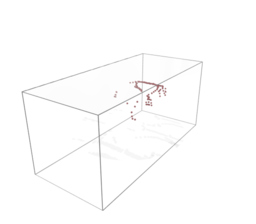
\includegraphics[width=3.75cm,trim={0.5cm 0 1cm 0.75cm},clip]{gfx/overview_small/points/00017}
    \end{subfigure}
    \begin{subfigure}[t]{0.20\textwidth}
        %\hspace*{-0.75cm}
        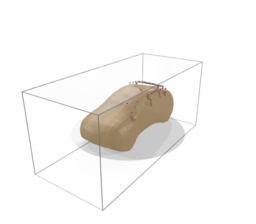
\includegraphics[width=3.75cm,trim={0.5cm 0 1cm 0.75cm},clip]{gfx/overview_small/sdf_points/00017}
    \end{subfigure}\\[-0.1cm]
    \begin{subfigure}[t]{0.5\textwidth}
        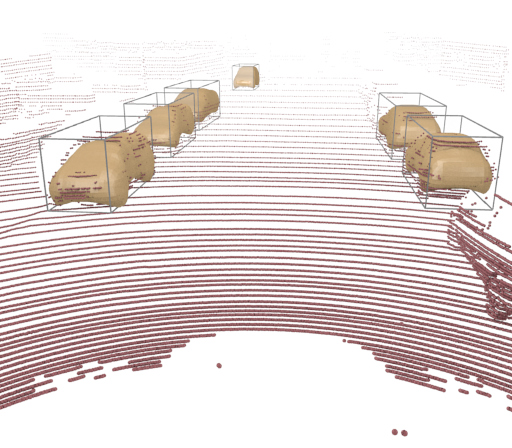
\includegraphics[width=8.25cm,trim={0 8cm 0cm 2cm},clip]{gfx/overview_small/00000}
    \end{subfigure}
    %\vspace*{-4px}
    \caption{{\bf Illustration of the 3D Shape Completion Problem.}
    %On top, we show the Velodyne point cloud of a street scene, annotated with the provided ground truth 3D bounding boxes.
    Top: Given a 3D bounding box and an incomplete point cloud (left, {\color{rred}red}), our goal is to predict the complete shape of the object (right, {\color{rbeige}beige}).
    % missing ground truth shapes.
    %e illustrate an extracted point clouds and the shape completion of our proposed method.
    Bottom: Shape completion results on a street scene from KITTI \cite{Geiger2012CVPR}.
    Learning shape completion on real-world data is challenging due to sparse / noisy observations and missing ground truth.}
    \label{fig:introduction}
    \vspace*{-0.25cm}
\end{figure}

3D shape perception is a long-standing problem both in human \cite{Pizlo2007CAIP,Pizlo2010} and computer vision \cite{Furukawa2013FTCGV}. In both disciplines, a large body of work focuses on 3D reconstruction, \eg, reconstructing objects or scenes from one or multiple views, which is an inherently ill-posed inverse problem where many configurations of shape, color, texture and lighting may result in the very same image \cite{Furukawa2013FTCGV}.
%In human vision, one of the fundamental problems is understanding how the human visual system accomplishes such tasks; in computer vision, in contrast, the goal is to develop 3D reconstruction systems.
Both human and computer vision are related through insights regarding the cues and constraints used by humans to perceive 3D shapes. Motivated by results from human vision \cite{Pizlo2007CAIP,Pizlo2010}, these priors are usually built into 3D reconstruction pipelines through explicit assumptions. Recently, however -- leveraging the success of deep learning -- researchers started to \emph{learn} shape models from data. Predominantly generative models have been used to learn how to generate, manipulate and reason about 3D shapes, \eg, \cite{Girdhar2016ECCV,Brock2016ARXIV,Sharma2016ARXIV,WuNIPS2016,Wu2015CVPR}, thereby offering many interesting possibilities for a wide variety of problems.

\begin{figure*}[t]
    \vspace*{-0.5cm}
	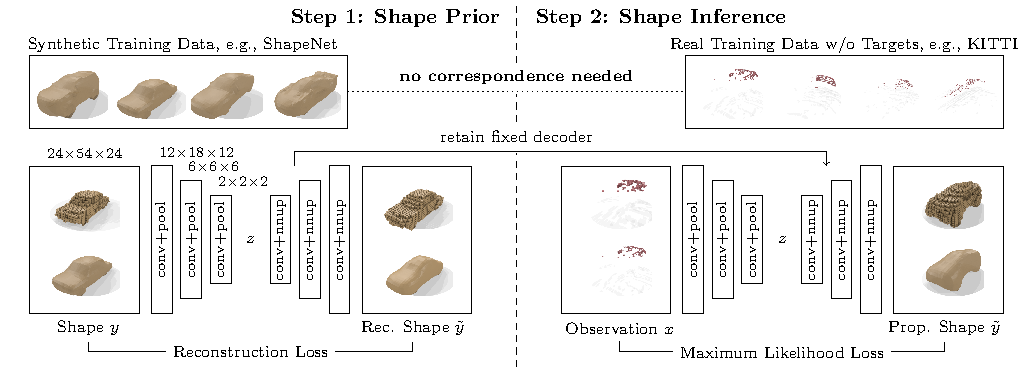
\includegraphics[width=\linewidth]{fig/overview_large}
    %\vspace*{-16px}
	\centering
    \caption{{\bf Proposed Amortized Maximum Likelihood (\AML) Approach to 3D Shape Completion.} We illustrate our amortized maximum likelihood (\AML) approach on KITTI \cite{Geiger2012CVPR}. We consider two steps. In step 1 (left), we use car models from ShapeNet \cite{Chang2015ARXIV} to train a variational auto-encoder (\VAE) \cite{Kingma2013ARXIV}. In our case, the car models are encoded using occupancy grids and signed distance functions (SDFs) at a resolution of $24 \times 54 \times 24$ voxels. In step 2 (right), we retain the pre-trained decoder (with fixed weights) and train a novel deterministic encoder. This network can be trained using a maximum likelihood loss without requiring further supervision. The pre-trained decoder constrains the predictions to valid car shapes while the maximum likelihood loss aligns the predictions with the observations. See text for further details.}
    \label{fig:method}
    \vspace*{-0.25cm}
\end{figure*}
%\documentclass[border=0pt]{standalone}
\usepackage{xcolor}
\usepackage{tikz,tikz-3dplot}
\begin{document}
	\tdplotsetmaincoords{50}{130}
    \begin{tikzpicture}
    % ---------------------------------------------------------
    \node at (5.2, 3.75) {{\bf Step 1: Shape Prior}};
    
    \node[rectangle,draw=black,anchor=west] (prior) at (-1,2.5) {
        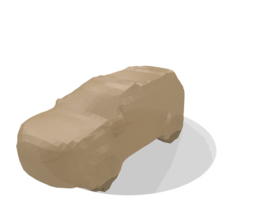
\includegraphics[height=1cm,trim={1cm 1.5cm 3.5cm 3cm},clip]{../gfx/overview_large/00010_target_off}
        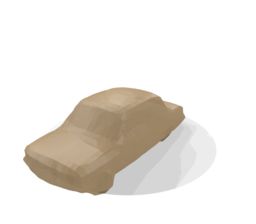
\includegraphics[height=1cm,trim={1cm 1.5cm 3.5cm 3cm},clip]{../gfx/overview_large/00004_target_off}
        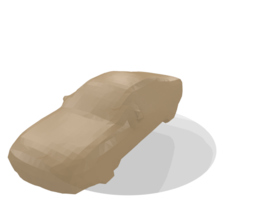
\includegraphics[height=1cm,trim={1cm 1.5cm 3.5cm 3cm},clip]{../gfx/overview_large/00000_target_off}
        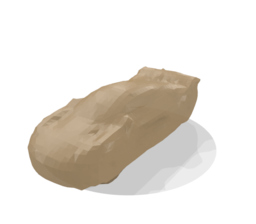
\includegraphics[height=1cm,trim={1cm 1.5cm 3.5cm 3cm},clip]{../gfx/overview_large/00012_target_off}
    };
    \node at (1.6,3.3) {\footnotesize Synthetic Training Data, e.g., ShapeNet};
    
    \node[] (y) at (0, -1.5) {\footnotesize Shape $y$};
    
    \node[rectangle,draw=black,anchor=west] (input) at (-1, 0) {
        \begin{tabular}{c}
            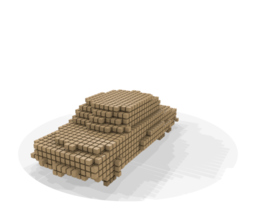
\includegraphics[height=1cm,trim={1cm 1.5cm 3.5cm 3cm},clip]{../gfx/overview_large/00004_target_binvox}\\
            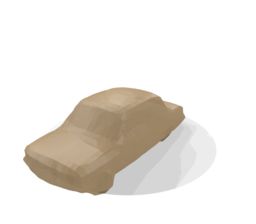
\includegraphics[height=1cm,trim={1cm 1.5cm 3.5cm 3cm},clip]{../gfx/overview_large/00004_target_off}
        \end{tabular}
    };  
    \node at ($(input.north) + (0,0.2)$) {\scriptsize $24{\times}54{\times}24$};
    
    \draw[-] ($(input.north east) + (0.2,0)$) rectangle ($(input.south east) + (0.55,0)$);
    \node[rotate=90] at ($(input.east) + (0.375,0)$) {\scriptsize conv+pool};
    \node[anchor=south west] at ($(input.north east) + (0.2,0)$) {\scriptsize $12{\times}18{\times}12$};
    \draw[-] ($(input.north east) + (0.7,-0.25)$) rectangle ($(input.south east) + (1.05,0.25)$);
    \node[rotate=90] at ($(input.east) + (0.875,0)$) {\scriptsize conv+pool};
    \node[anchor=south west] at ($(input.north east) + (0.7,-0.25)$) {\scriptsize $6{\times}6{\times}6$};
    \draw[-] ($(input.north east) + (1.2,-0.5)$) rectangle ($(input.south east) + (1.55,0.5)$);
    \node[rotate=90] at ($(input.east) + (1.375,0)$) {\scriptsize conv+pool};
    \node[anchor=south west] at ($(input.north east) + (1.2,-0.5)$) {\scriptsize $2{\times}2{\times}2$};
    
    \node (z) at (2.75, 0) {\footnotesize $z$};
    
    \node[rectangle,draw=black,anchor=east] (output) at (6.5, 0) {
        \begin{tabular}{c}
        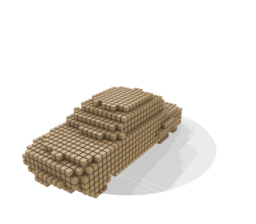
\includegraphics[height=1cm,trim={1cm 1.5cm 3.5cm 3cm},clip]{../gfx/overview_large/00004_prediction_binvox}\\
        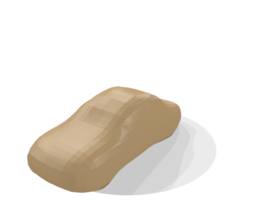
\includegraphics[height=1cm,trim={1cm 1.5cm 3.5cm 3cm},clip]{../gfx/overview_large/00004_prediction_off}
        \end{tabular}
    };
    
    \draw[-] ($(output.north west) - (0.2,0)$) rectangle ($(output.south west) - (0.55,0)$);
    \node[rotate=90] at ($(output.west) - (0.375,0)$) {\scriptsize conv+nnup};
    \draw[-] ($(output.north west) - (0.7,0.25)$) rectangle ($(output.south west) - (1.05,-0.25)$);
    \node[rotate=90] at ($(output.west) - (0.875,0)$) {\scriptsize conv+nnup};
    \draw[-] ($(output.north west) - (1.2,0.5)$) rectangle ($(output.south west) - (1.55,-0.5)$);
    \node[rotate=90] at ($(output.west) - (1.375,0)$) {\scriptsize conv+nnup};
    
    \node (ry) at (5.5, -1.5) {\footnotesize Rec. Shape $\tilde{y}$};
    
    \node[] (L) at (2.75, -1.9) {\footnotesize Reconstruction Loss};
    
    \draw[-] (ry) -- ($(ry) - (0,0.4)$);
    \draw[-] ($(ry) - (0,0.4)$) -- (L);
    \draw[-] (y) -- ($(y) - (0,0.4)$);
    \draw[-] ($(y) - (0,0.4)$) -- (L);
    
    % --
    \draw[-] (3.5, 1.25) -- (3.5, 1.5);
    \draw[-] (3.5, 1.5) -- (12.5, 1.5);
    \draw[->] (12.5, 1.5) -- (12.5, 1.25);
    \node at (7.25, 1.75) {\footnotesize retain fixed decoder};
    \draw[-,dashed] (7.25,-2.15) -- (7.25,1.45);
    \draw[-,dashed] (7.25,2) -- (7.25,2.45);
    \draw[-,dashed] (7.25,3) -- (7.25,4.05);
    
    \node at (7.25, 2.75) {\footnotesize\textbf{no correspondence needed}};
    \begin{scope}[shift={(9,0)}]
    
    % ---------------------------------------------------------
    \node at (0.7, 3.75) {{\bf Step 2: Shape Inference}};
    
    \node[rectangle,draw=black,anchor=east] (inference) at (6.5,2.5) {
        
\includegraphics[height=1cm,trim={1cm 1.5cm 3.5cm 3cm},clip]{../gfx/overview_large/00037_input_txt}
        
\includegraphics[height=1cm,trim={1cm 1.5cm 3.5cm 3cm},clip]{../gfx/overview_large/00005_input_txt}
        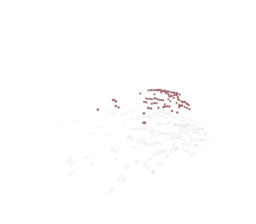
\includegraphics[height=1cm,trim={1cm 1.5cm 3.5cm 3cm},clip]{../gfx/overview_large/00045_input_txt}
        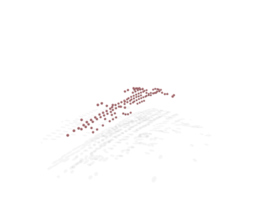
\includegraphics[height=1cm,trim={1cm 1.5cm 3.5cm 3cm},clip]{../gfx/overview_large/00047_input_txt}
    };
    \node at (3.8,3.3) {\footnotesize Real Training Data w/o Targets, e.g., KITTI};
    
    % --
    \draw[-,dotted] (prior) -- (inference);
    
    \node[] (y) at (0, -1.5) {\footnotesize Observation $x$};
    
    \node[rectangle,draw=black,anchor=west] (input) at (-1, 0) {
        \begin{tabular}{c}
        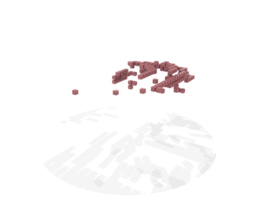
\includegraphics[height=1cm,trim={1cm 1.5cm 3.5cm 3cm},clip]{../gfx/overview_large/00037_input_binvox}\\
        
\includegraphics[height=1cm,trim={1cm 1.5cm 3.5cm 3cm},clip]{../gfx/overview_large/00037_input_txt}
        \end{tabular}
    };
    
    \draw[-] ($(input.north east) + (0.2,0)$) rectangle ($(input.south east) + (0.55,0)$);
    \node[rotate=90] at ($(input.east) + (0.375,0)$) {\scriptsize conv+pool};
    \draw[-] ($(input.north east) + (0.7,-0.25)$) rectangle ($(input.south east) + (1.05,0.25)$);
    \node[rotate=90] at ($(input.east) + (0.875,0)$) {\scriptsize conv+pool};
    \draw[-] ($(input.north east) + (1.2,-0.5)$) rectangle ($(input.south east) + (1.55,0.5)$);
    \node[rotate=90] at ($(input.east) + (1.375,0)$) {\scriptsize conv+pool};
    
    \node (z) at (2.75, 0) {\footnotesize $z$};
    
    \node[rectangle,draw=black,anchor=east] (output) at (6.5, 0) {
        \begin{tabular}{c}
        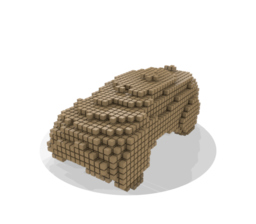
\includegraphics[height=1cm,trim={1cm 1.5cm 3.5cm 3cm},clip]{../gfx/overview_large/00037_prediction_binvox}\\
        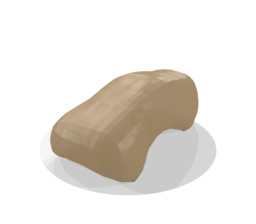
\includegraphics[height=1cm,trim={1cm 1.5cm 3.5cm 3cm},clip]{../gfx/overview_large/00037_prediction_off}
        \end{tabular}
    };
    
    \draw[-] ($(output.north west) - (0.2,0)$) rectangle ($(output.south west) - (0.55,0)$);
    \node[rotate=90] at ($(output.west) - (0.375,0)$) {\scriptsize conv+nnup};
    \draw[-] ($(output.north west) - (0.7,0.25)$) rectangle ($(output.south west) - (1.05,-0.25)$);
    \node[rotate=90] at ($(output.west) - (0.875,0)$) {\scriptsize conv+nnup};
    \draw[-] ($(output.north west) - (1.2,0.5)$) rectangle ($(output.south west) - (1.55,-0.5)$);
    \node[rotate=90] at ($(output.west) - (1.375,0)$) {\scriptsize conv+nnup};
    
    \node (ry) at (5.5, -1.5) {\footnotesize Prop. Shape $\tilde{y}$};
    
    \node[] (L) at (2.75, -1.9) {\footnotesize Maximum Likelihood Loss};
    
    \draw[-] (ry) -- ($(ry) - (0,0.4)$);
    \draw[-] ($(ry) - (0,0.4)$) -- (L);
    \draw[-] (y) -- ($(y) - (0,0.4)$);
    \draw[-] ($(y) - (0,0.4)$) -- (L);
    \end{scope}
    \end{tikzpicture}
\end{document}


In this paper, we focus on the problem of inferring and completing 3D shapes based on sparse and noisy 3D point observations as illustrated in \figref{fig:introduction}.
%This problem has many relevant applications, including 
This problem occurs when only a single view of an individual object is provided or large parts of the object are occluded as, \eg, in autonomous driving applications.
%The problem is, however, also closely related to surface reconstruction \cite{Berger2014EUROGRAPHICS} and, thus, has relevant applications in computer graphics, as well.
Existing approaches to shape completion can be roughly categorized into data-driven and learning-based methods. The former usually rely on learned shape priors and formulate shape completion as optimization problem over the corresponding (lower-dimensional) latent space \cite{Engelmann2016GCPR,Bao2013CVPR,Dame2013CVPR,Guney2015CVPR}. These approaches have demonstrated impressive performance on real data, \eg, on KITTI \cite{Geiger2012CVPR}.
% as demonstrated in \cite{Engelmann2016GCPR}.
Learning-based approaches, in contrast, assume a fully supervised setting in order to directly learn shape completion on synthetic data \cite{Riegler2017THREEDV,SmithARXIV2017,Dai2017CVPRa,Sharma2016ARXIV,Fan2016ARXIV,Rezende2016ARXIV}. As full supervision is required, the applicability of these approaches to real data is limited.
% and has -- to the best of our knowledge -- not been addressed.
However, learning-based approaches offer advantages in terms of efficiency: a forward pass of the learned network is usually sufficient. In practice, both problems -- the optimization problem of data-driven approaches and the required supervision of learning-based approaches -- limit the applicability of state-of-the-art shape completion methods to real data.

%In this work, we propose a model which tackles this problem.
%address both problems: the need of annotated training data and the drawbacks of computationally involved optimization problems.
%In particular, we utilize ShapeNet \cite{Chang2015ARXIV} to learn a strong shape prior using variational auto-encoders \cite{Kingma2013ARXIV}.

% ag: add something of this again?
%We hypothesize that using a strong prior of possible shapes allows us to learn shape completion under weak supervision, \ie, only given knowledge about the object category at hand. On real data, we additionally assume knowledge about the object location in the form of bounding boxes which can be provided by an object detector.
%
%By learning shape completion using deep networks, we additionally reduce the problem to a forward pass of the trained network. 
%{\color{red} Question: can I stop citing a paper after I first cited it (except for related work)?}
% ag: yes.
%\textbf{Contribution.}
%
To tackle these problems, this work proposes an amortized maximum likelihood approach for 3D shape completion.
More specifically, we first learn a shape model on synthetic data using a variational auto-encoder \cite{Kingma2013ARXIV} (\cf Figure \ref{fig:method}, step 1). Shape completion can then be formulated as maximum likelihood problem -- in the spirit of \cite{Engelmann2016GCPR}.
Instead of maximizing the likelihood independently for distinct observations, however, we follow the idea of amortized inference \cite{Gersham2014COGSCI} and \emph{learn} to predict the maximum likelihood solutions directly given the observations.
Towards this goal, we train a new encoder which embeds the observations in the same latent space using an unsupervised maximum likelihood loss (\cf Figure \ref{fig:method}, step 2). This allows us to learn 3D shape completion in challenging real-world situations, \eg, on KITTI.
Using signed distance functions to represent shapes, we are able to obtain sub-voxel accuracy while applying regular 3D convolutional neural networks to voxel grids of limited resolution, yielding a highly efficient inference method.
For experimental evaluation, we introduce two novel, synthetic shape completion benchmarks based on ShapeNet and ModelNet. On KITTI, we further compare our approach to the work of Engelmann \etal \cite{Engelmann2016GCPR} -- the only related work which addresses shape completion on KITTI.
Our experiments demonstrate that we obtain shape reconstructions which rival data-driven techniques while significantly reducing inference time.
Our code and datasets are made publicly available\footnote{\url{https://avg.is.tuebingen.mpg.de/research_projects/3d-shape-completion}.}.
%The presented experiments support our claim that shape completion can be learned  shape priors allow weakly-supervised learning of shape completion.

This paper is structured as follows: we discuss related work in Section \ref{sec:related-work}. In Section \ref{sec:method} we describe our amortized maximum likelihood framework for weakly-supervised shape completion. We present experimental results in Section \ref{sec:experiments} and conclude in Section \ref{sec:conclusion}.

\section{Related Work}
\label{sec:related-work}

\boldparagraph{Symmetry-based and Data-driven Methods}
%
Shape completion is usually performed on partial scans of individual objects. Following \cite{SungTG2015}, classical shape completion approaches can roughly be categorized into symmetry-based methods and data-driven methods. The former leverage observed symmetry to complete shapes; representative works include \cite{ThrunICCV2005,PaulyTG2008,ZhengTG2010,KroemerHUMANOIDS2012,LawCVIU2011}.
The data-driven case is more interesting in relation to the proposed approach.
In early work, Pauly \etal \cite{Pauly2005SGP} pose shape completion as retrieval and alignment problem.
In \cite{LiCGF2015,Engelmann2016GCPR,Engelmann2017WACV,Nan2012TG,Bao2013CVPR,Dame2013CVPR,Gupta2015CVPR} shape retrieval is avoided by learning a latent shape space.
The alignment task is then posed as an optimization problem over the latent shape variables.
Data-driven approaches are applicable to real data assuming knowledge about the category of shapes in order to learn the shape prior.
However, they require costly optimization at inference time. In contrast, we propose an approach which amortizes the inference procedure by means of a deep neural network allowing for efficient completion of 3D shapes.

%Engelmann \etal \cite{Engelmann2016GCPR} considers the problem of shape completion on the challenging KITTI dataset \cite{Geiger2012CVPR} using a learned shape prior.

\boldparagraph{Learning-based Methods}
%
With the recent success of deep learning, several learning-based approaches have been proposed \cite{Firman2016CVPR,SmithARXIV2017,Dai2016ARXIV,Sharma2016ARXIV,Rezende2016ARXIV,Fan2016ARXIV,Riegler2017THREEDV,Han2017ICCV}. Strictly speaking, those techniques are data-driven as well, however, shape retrieval and fitting is avoided by learning shape completion under full supervision on synthetic datasets such as ShapeNet \cite{Chang2015ARXIV} or ModelNet \cite{Wu2015CVPR} -- usually using deep neural networks.
%Most of them use deep neural networks to learn shape completion under full supervision on synthetic datasets such as ShapeNet \cite{Chang2015ARXIV} or ModelNet \cite{Wu2015CVPR}.
Some approaches \cite{Riegler2017THREEDV,Haene2017ARXIV,Tatarchenko2017ICCV} use octrees to predict high-resolution shapes via supervision provided at multiple scales.
% but the applicability (or generalization) to real data has -- to the best of our knowledge -- not been studied so far.
However, full supervision for the 3D shape is often not available in real-world situations (\eg, KITTI \cite{Geiger2012CVPR}), thus existing models are primarily evaluated on synthetic datasets.
In this paper, we propose to train a shape prior on synthetic data, but leverage unlabeled real-world data for learning shape completion. %\green{Additionally}, our model also handles implicit surface representations leading to sub-voxel accuracy instead of simple occupancy representations.

%%%%%%%%%%%%%%%%%%%%%%%%%%%%%%%%
% ag: the following section doesn't fit as is. some of the papers have been cited, but otherwise the paragraph would need to be reworked to fit the story. commented out for now.

%\boldparagraph{Shape Priors}
%%
%For shape completion, learning-based approaches can be understood as implicitly learning a shape prior from training data \cite{SmithARXIV2017,Dai2016ARXIV,Sharma2016ARXIV,Rezende2016ARXIV}. To avoid explicitly aligning and retrieving shapes, data-driven approaches also use learned shape priors \cite{Engelmann2016GCPR,Engelmann2017WACV}. However, shape priors have also been applied in different domains, \eg, in 3D pose estimation \cite{Prisacariu2013ACCV,AdrianACCV2012,Dambreville2008PAMI,SandhuCVPR2009,Menze2015ISA} or tracking \cite{Ma2014ECCV,LeottaCVPR2009}. In classical 3D reconstruction, shape priors are also commonly used to resolve ambiguities \cite{Guney2015CVPR}, specularities \cite{Dame2013CVPR} or simply incomplete observations \cite{Bao2013CVPR,Engelmann2016GCPR,Engelmann2017WACV}. In the context of shape modeling, deep generative models such as variational auto-encoders \cite{Kingma2013ARXIV} or generative adversarial networks \cite{Goodfellow2014NIPS} have been used to generate, manipulate and reason about shapes \cite{Sharma2016ARXIV,Dai2016ARXIV,Girdhar2016ECCV,WuNIPS2016,Wu2015CVPR,SmithARXIV2017}. In our case, a learned shape prior has the primary purpose to constrain the space of possible shapes in order to enable weakly-supervised learning.

%\textbf{3D Generative Models.} Recently, generative deep models received considerable attention, \eg, \cite{VanDenOordICML2016,VanDenOordNIPS2016,Goodfellow2014NIPS,MakhzaniARXIV2015,Kingma2013ARXIV,LarsenICML2016}. In this work, we resort to variational auto-encoders \cite{Kingma2013ARXIV} as generative adversarial networks are known to be harder to train \cite{MeschederARXIV2017,NowozinNIPS2016,Salimans2016NIPS}. We are not the first to make use of these models; related works include \cite{Sharma2016ARXIV,Dai2016ARXIV,Girdhar2016ECCV,WuNIPS2016,Wu2015CVPR,SmithARXIV2017} where generative models are usually used to learn a low-dimensional latent space of shapes.


\boldparagraph{Amortized Inference}
%
The notion of amortized inference was introduced in \cite{Gersham2014COGSCI} and exploited repeatedly in recent work \cite{RezendeICML2015,WangARXIV2016,RitchieARXIV2016}. Generally, it describes the idea of \emph{learning how to infer}; in our case, we learn, \ie amortize, the maximum likelihood inference problem by training a network to directly predict maximum likelihood solutions.
\section{Method}
\label{sec:method}

In the following, we first introduce the mathematical formulation of the weakly-supervised 3D shape completion problem. Subsequently, we briefly discuss the concept of variational auto-encoders (\VAEs) \cite{Kingma2013ARXIV} which we use to learn a shape prior.
% -- which are used to learn a shape prior based on the reference shapes.
Finally, we formally derive our proposed amortized maximum likelihood (\AML) approach. The overall framework is also illustrated in Figure \ref{fig:method}.

\subsection{Problem Formulation}

In a supervised setting, our task can be described as follows: given a set of partial observations $\mathcal{X} = \{x_n\}_{n = 1}^N \subseteq \mathbb{R}^R$ and corresponding ground truth shapes $\mathcal{Y}^* = \{y_n^*\}_{n = 1}^N \subseteq \mathbb{R}^R$, learn a mapping $x_n \mapsto y_n^*$ that is able to generalize to previously unseen observations. Here, we assume $\mathbb{R}^R$ to be a suitable vector representation of observations and shapes; in practice, we resort to occupancy grids or signed distance functions (SDFs) defined on regular grids, \ie, $x_n, y_n^* \in \mathbb{R}^{H \times W \times D} \simeq \mathbb{R}^R$.
SDFs represent the distance of each voxel's center to the closest point on the surface; we use negative signs for interior voxels.
For the (partial) observations, we write $x_n \in \{0, 1, \uk\}^R$ to make missing information explicit; in particular, $x_{n,i} = \uk$ corresponds to unobserved voxels, while $x_{n,i} = 1$ and $x_{n,i} = 0$ correspond to occupied and unoccupied voxels, respectively.

On real data, \eg, KITTI \cite{Geiger2012CVPR}, supervised learning is often not possible as obtaining ground truth annotations is labor intensive (\eg, \cite{Menze2015CVPR,Xie2016CVPR}). Therefore, we target a weakly-supervised variant of the problem instead. Given observations $\mathcal{X}$ and a set of reference shapes $\mathcal{Y} = \{y_m\}_{m = 1}^M \subseteq \mathbb{R}^R$ both of the same, known object category, learn a mapping $x_n \mapsto \tilde{y}(x_n)$ such that the predicted shape $\tilde{y}(x_n)$ matches the unknown ground truth shape $y_n^*$ as close as possible.
Here, supervision is provided in the form of the known object category, allowing to derive the reference shapes from (watertight) triangular meshes; on real data, we also assume the object locations to be given in the form of 3D bounding boxes in order to extract the observations $\mathcal{X}$.
%\green{In practice, the reference shapes $\mathcal{Y}$ are derived from watertight, triangular meshes in order to obtain well-defined occupancy grids and SDFs.}
%In the following, we assume that the shapes $\mathcal{Y}$ are available as meshes from which we derive occupancy grids and SDFs; the observations are voxelized as described above.

\subsection{Shape Prior}
\label{subsec:method-prior}

We propose to use the provided reference shapes $\mathcal{Y}$ to learn a model of possible 3D shapes over the latent space $\mathcal{Z} = \mathbb{R}^Q$ with $Q \ll R$. The prior model is learned using a \VAE where the joint distribution $p(y, z)$ decomposes into $p(y, z) = p(y | z)p(z)$ with $p(z)$ being a unit Gaussian, \ie, $p(z) = \mathcal{N}(z;0, I_Q)$ with $I_Q \in \mathbb{R}^{R \times R}$ being the identity matrix. Sampling from the model is then performed by choosing $z \sim p(z)$ and subsequently sampling $y \sim p(y | z)$. For training the generative model, we also need to approximate the posterior $q(z | y) \approx p(z | y)$, \ie, the inference model. In the framework of the variational auto-encoder, both the so-called recognition model $q(z | y)$ and the generative model $p(y | z)$ -- corresponding to encoder and decoder -- are represented by neural networks. In particular,
\begin{align}
%\text{\bf Encoder: }
q(z | y) = \mathcal{N}(z_i; \mu_i(y), \text{diag}(\sigma_i^2(y)))
\end{align}
where $\mu(y), \sigma^2(y) \in \mathbb{R}^Q$ are predicted using the encoder neural network and $p(y_i | z)$ is assumed to be a Bernoulli distribution when working with occupancy grids, \ie, $p(y_i | z) = \text{Ber}(y_i ; \theta_i(z))$ while a Gaussian distribution is used when predicting SDFs, \ie, $p(y_i | z) = \mathcal{N}(y_i ; \mu_i(z), \sigma^2)$. In both cases, the parameters, \ie, $\theta_i(z)$ or $\mu_i(z)$, are predicted using the decoder neural network. For SDFs, we neglect the variance ($\sigma^2 = 1$) as it merely scales the training objective.

In the framework of variational inference, the parameters of the encoder and the decoder are found by maximizing the likelihood $p(y)$. In practice, the likelihood is often intractable. Instead, the evidence lower bound is maximized, resulting in the following loss to be minimized:
\begin{align}
\mathcal{L}_{\text{VAE}}(w) = - \mathbb{E}_{q(z |y)}[\ln p(y|z)] + \text{KL}(q(z | y)| p(z)).
\end{align}
where $w$ are the weights of the encoder and decoder. The Kullback-Leibler divergence $\text{KL}$ can be computed analytically; the expectation corresponds to a binary cross-entropy error for occupancy grids or a scaled sum-of-squared error for SDFs. The loss $\mathcal{L}_{\text{VAE}}$ is minimized using stochastic gradient descent (SGD). We refer to \cite{Kingma2013ARXIV} for details.

\subsection{Shape Inference}
\label{subsec:method-inference}

After learning the shape prior $p(y, z) = p(y| z) p(z)$, shape completion can be formulated as a maximum likelihood (\ML) problem over the lower-dimensional latent space $\mathcal{Z} = \mathbb{R}^Q$. The corresponding negative log-likelihood, \ie, $-\ln p(y, z)$, can be written as
%
\begin{align}
\mathcal{L}_{\text{ML}}(z) &= - \sum_{x_i \neq \uk} \ln p(y_i = x_i | z) - \ln p(z).\label{eq:ml}
\end{align}
%
where $x_i \neq \uk$ expresses that the summation ranges only over observed voxels.
As the prior $p(z)$ is Gaussian, the corresponding negative log-probability $- \ln p(z) \propto \|z\|_2^2$ results in a quadratic regularizer. As before, the generative model $p(y | z)$ decomposes over voxels.
% here, we can only consider actually observed voxels, \ie, $x_i \neq \uk$.
Instead of solving Equation \eqref{eq:ml} for each observation $x \in \mathcal{X}$ individually, we follow the idea of amortized inference \cite{Gersham2014COGSCI} and train an encoder $z(x;w)$ to \emph{learn} \ML. To this end, we keep the generative model $p(y|z)$ fixed and train the weights $w$ of the encoder $z(x;w)$ using the \ML objective as loss:
%
\begin{align}
\mathcal{L}_{\text{AML}}(w) = - \sum _{x_i \neq \uk} \ln p(y_i = x_i | z) - \lambda \ln p(z).\label{eq:aml}
\end{align}
%
where we added an additional parameter $\lambda$ controlling the importance of the shape prior. The exact form of the probabilities $p(y_i = x_i | z)$ depends on the used shape representation. In the case of occupancy grids, this term results in a cross-entropy error (as both $y_i$ and $x_i$ are, for $x_i \neq \uk$, binary). However, when using SDFs, the term is not well-defined as $p(y_i | z)$ is modeled with a continuous Gaussian distribution, while the observations $x_i$ are binary, \ie, it is unclear how to define $p(y_i = x_i | z)$. Alternatively, we could derive distance values along the rays corresponding to observed points (\eg, following \cite{Steinbrucker2013ICCV}). However, as illustrated in Figure \ref{fig:method-sdf}, noisy rays lead to invalid observations along the whole ray. This problem can partly be avoided when relying on occupancy to represent the observations.

\begin{figure}
    \centering
    \vspace*{-0.25cm}
    \begin{subfigure}[t]{0.425\linewidth}
        \vspace{0px}
        \centering
        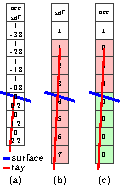
\includegraphics[width=1\linewidth]{fig/method_sdf_2}
    \end{subfigure}
    \hfill
    \begin{subfigure}[t]{0.5\linewidth}
        \vspace{3px}
        \centering
        \hspace*{-12px}
        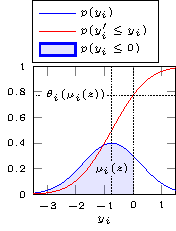
\includegraphics[width=1\linewidth]{fig/method_sdf_1}
    \end{subfigure}
    \vspace*{-10px}
    \caption{{\bf Left: Problem when Predicting SDFs.} Illustration of a ray ({\color{red}red}) correctly hitting a surface ({\color{blue}blue}) causing the SDF values and occupancy values in the underlying voxel grid to be correct (\cf (a)). A noisy ray, however, causes all voxels along the ray to get invalid distances assigned (marked {\colorbox{red!25}{red}}; \cf (b)). When using occupancy, in contrast, only the voxels behind the surface are assigned invalid occupancy states (marked {\colorbox{red!25}{red}}); the remaining voxels are labeled correctly (marked {\colorbox{green!25}{green}}; \cf (c)).
    {\bf Right: Proposed Gaussian-to-Bernoulli Transformation.} For $p(y_i) := p(y_i | z) = \mathcal{N}(y_i;\mu_i(z), \sigma^2)$ ({\color{blue}blue}), we illustrate the transformation discussed in Section \ref{subsec:method-inference}, allowing to use the binary observations $x_i$ (for $x_i \neq \uk$) to supervise the SDF predictions. This is achieved, by transforming the predicted Gaussian distribution to a Bernoulli distribution with occupancy probability $\theta_i(\mu_i(z)) = p(y_i \leq 0)$ ({\color{blue}blue area}).}
    \label{fig:method-sdf}
    \vspace*{-0.25cm}
\end{figure}

In order to still work with SDFs (to achieve sub-voxel accuracy) we propose to define $p(y_i = x_i | z)$ through a simple transformation. In particular, as $p(y_i | z)$ is modeled as Gaussian distribution $p(y_i | z) = \mathcal{N}(y_i ; \mu_i(z), \sigma^2)$ where $\mu_i(z)$ is predicted using the fixed decoder (and $\sigma^2 = 1$) and $x_i$ is binary (for $x_i \neq \uk$), we introduce a mapping $\theta_i(\mu_i(z))$ transforming the predicted Gaussian distribution to a Bernoulli distribution with occupancy probability $\theta_i(\mu_i(z))$, \ie, $p(y_i = x_i|z)$ becomes $\text{Ber}(y_i = x_i; \theta_i(\mu_i(z)))$.
%
%ag: no need to discuss this I think
%This is necessary, as the observation $x_i \neq \uk$ is inherently binary. Although we could derive distance functions from the observations, \eg, along the rays corresponding to observed points \ag{You had a paper here, right?}, even slight noise can result in large changes in the derived distances (along the whole ray). 
%
%\begin{align}
%p(y_i = x_i | z) = \text{Ber}(y_i = x_i; \theta_i(\mu_i(z)))
%\end{align}
As we defined occupied voxels to have negative sign in the SDF, we can derive the occupancy probability $\theta_i(\mu_i(z))$ as the probability of a negative distance:
\begin{align}
\theta_i(\mu_i(z)) &= \mathcal{N}(y_i \leq 0; \mu_i(z), \sigma^2)\label{eq:sdf}\\
%& = \int_{y_i'}^0 \mathcal{N}(y_i' \leq 0; \mu_i(z), \sigma^2) dy_i'\\
&= \frac{1}{2} \left(1 + \text{erf}\left(\frac{- \mu_i(z)}{\sigma \sqrt{\pi}}\right)\right).\label{eq:sdf-erf}
\end{align}
%
Here, $\text{erf}$ is the error function which, in practice, is approximated following \cite{Abramowitz1974}. Equation \eqref{eq:sdf} is illustrated in Figure~\ref{fig:method-sdf} where the occupancy probability $\theta_i(\mu_i(z))$ is computed as the area under the Gaussian bell curve for $y_i \leq 0$. This per-voxel transformation can easily be implemented as non-linearity layer and its derivative \wrt $\mu_i(z)$ is -- by construction -- a Gaussian distribution. Overall, this transformation allows to predict SDFs while using binary observations.
\section{Experimental Evaluation}
\label{sec:experiments}

In this section, we present quantitative and qualitative experimental results. First, we derive a synthetic benchmark for 3D shape completion of cars based on ShapeNet \cite{Chang2015ARXIV}. Second, we present results on KITTI \cite{Geiger2012CVPR} and compare the proposed amortized maximum likelihood (\AML) approach to the data-driven approach of \cite{Engelmann2016GCPR}.
We also consider regular maximum likelihood (\ML) and a fully-supervised model (\Sup; following related work \cite{Dai2016ARXIV,Sharma2016ARXIV,Riegler2017THREEDV,Han2017ICCV}) as baselines.
%While our synthetic benchmark naturally includes ground truth shapes, KITTI does not include any ground truth shapes. To demonstrate the benefits of \AML,
Finally, we consider additional object categories on ModelNet \cite{Wu2015CVPR}.
We provide complementary details and experiments in the supplementary material.
% In the following, we discuss the used datasets, architecture and training, evaluation measures and relevant baselines.

\subsection{Datasets}
\label{subsec:experiments-data}

\boldparagraph{ShapeNet}
%
On ShapeNet, we took $3253$ car models, and simplified them using the approach outlined in \cite{Guney2015CVPR} to obtain watertight meshes. \green{After random translation, rotation and scaling, we extract two sets: the reference shapes $\mathcal{Y}$ and the ground truth shapes $\mathcal{Y}^*$ (such that $\mathcal{Y} \cap \mathcal{Y}^* = \emptyset$).}
To train the shape prior using the reference shapes $\mathcal{Y}$, we derive signed distance functions (SDFs) and occupancy grids at a resolution of $24 \times 54 \times 24$ voxels. \green{The ground truth shapes~$\mathcal{Y}^*$ are rendered to obtain the observations $\mathcal{X}$}. In particular, we identify occupied voxels, \ie, $x_{n,i} = 1$, by back-projecting pixels from the rendered depth image and perform ray tracing to identify free space, \ie, $x_{n,i} = 0$ (all other voxels are unknown, \ie, $x_{n,i} = \uk$).

In order to benchmark 3D shape completion, we consider two difficulties: a ``clean'' -- or easy -- version with depth images rendered at a resolution of $48 \times 64$ pixels and a ``noisy'' -- or hard -- version using a resolution of $24 \times 32$. On average, this results in $411$ and $106$ observed points (not necessarily voxels), respectively.
%Note that typically, a laser-based sensor installed, \eg, on an autonomous vehicle, does not provide more observations than this. Second, we also introduce a ``noisy'' -- or hard -- version. Here, we reduce the resolution of the captured depth images to $24 \times 32$ resulting in an average of only $106$ points being observed.
%Additionally, we inject noise: we add an exponentially-distributed error term (with rate parameter $70$) to every depth value; and randomly (with probability $0.075$) set depth values to the maximum depth.
\green{For the latter variant, we additionally inject noise by (randomly) perturbing pixels or setting them to the maximum depth value to simulate rays (\eg, from a LiDAR sensor) passing through objects (\eg, due to specular or transparent surfaces).}
%Overall, we obtain the reference shapes as training set for the shape prior, the ground truth shapes and the corresponding observations as training set for shape completion and similarly an additional validation set.
We refer to the created datasets as \clean and \noisy and show examples in Figure~\ref{fig:experiments-shapenet-kitti}.
\green{Overall, we obtain $14640$/$14640$/$1950$ samples for the prior training/inference training/validation set with roughly $1.06\%$/$0.32\%$ observed voxels and $7.04\%$/$4.8\%$ free space voxels for \clean/\noisy.}
\green{As can be seen, \clean and \noisy include a large variety of car models and \noisy, in particular, captures the difficulty of real data, \eg from KITTI, by explicitly modeling sparsity and noise.}

\boldparagraph{KITTI}
%
On KITTI, we extract observations using the provided ground truth 3D bounding boxes to avoid the inaccuracies of 3D object detectors.
%Note that while significant pr. While we also consider detections from \cite{Chen2016ARXIV}, as done similarly in \cite{Engelmann2016GCPR}, we found that most 3D object detectors still perform poorly on KITTI's 3D object detection benchmark\footnote{\url{http://www.cvlibs.net/datasets/kitti/eval_object.php?obj_benchmark=3d}}.
We used KITTI's Velodyne point clouds from the 3D object detection benchmark and the training/validation split of \cite{Chen2016ARXIV} ($7140$/$7118$ samples). Based on the average aspect ratio of cars in the dataset, we voxelize the points within the 3D bounding boxes into occupancy grids of size $24 \times 54 \times 24$ and perform ray tracing to obtain the observations $\mathcal{X}$.
% Based on statistics from the ground truth 3D bounding boxes on KITTI, we determined $H \times W \times D$ to be $24 \times 54 \times 24$.
%Depending on the distance from the sensor, some of the 3D bounding boxes contain only few points such that the derived observations are very sparse.
We filtered the observations to contain at least $50$ observed points to avoid overly sparse observations. On average, we obtained $0.3\%$ observed voxels and $3.35\%$ free space voxels. For the bounding boxes in the validation set, we generated partial ground truth by considering $10$ future and $10$ past frames and accumulating the corresponding 3D points according to the ground truth bounding boxes. In Figure \ref{fig:experiments-shapenet-kitti}, we show  examples of the extracted observations and ground truth. Overall, the extracted observations are very sparse and noisy and ground truth is not available for every observation.

\boldparagraph{ModelNet}
%
\green{On ModelNet, we consider the object categories bathtub, dresser, monitor, nightstand, sofa and toilet. We use a resolution of $32 \times 32 \times 32$ (similar to \cite{Wu2015CVPR}) and rely purely on occupancy grids as thin structures make SDFs unreliable in low resolution. Reference shapes $\mathcal{Y}$, ground truth shapes $\mathcal{Y}^\ast$ and observations $\mathcal{X}$ are obtained following the procedure for \clean (without simplification of the models). This results in -- on average -- $1.04\%$ observed voxels and $7.24\%$ free space voxels. Overall, we obtained a minimum of $700$/$700$/$150$ samples for prior training/inference training/validation per category. The large intra-category variations contribute to the difficulty of the task on ModelNet; we show examples in Figure \ref{fig:experiments-modelnet}.}

\subsection{Architecture and Training}
\label{subsec:experiments-architecture}

\begin{table*}
    \centering
    \vspace*{-0.25cm}
    {\small
    \begin{tabularx}{1\textwidth}{|X|ccc|ccc|c|c|}
        \hline
        & \multicolumn{3}{c|}{\clean (val)}
        & \multicolumn{3}{c|}{\noisy (val)}
        & KITTI (val)&\\
        & \Abs & \Acc [vx] & \Compl [vx] & \Abs & \Acc [vx] & \Compl [vx] & \Compl [m] & t [s]\\
        \hline\hline
        %\PPCA $Q{=}5$ & 0.03 & 0.51& 0.766137 &&&&&\\
        \PPCA & 0.025 & 0.41 & 0.628 &&&&&\\
        %\VAE $Q{=}5$ & 0.021 & 0.409 & 0.606 &&&&&\\
        \VAE & \bf 0.014 & \bf 0.283 & \bf 0.439 &&&&&\\
        \hline\hline
        \Mean & 0.068 & 1.33 & 1.576 & 0.068 & 1.33 & 1.576 && \bf 0\\
        \ML & 0.04 & 0.733 & 0.845 & 0.059 & 1.145 & 1.331 && 30\\
        \Sup (on KITTI GT) & \bf 0.022 & \bf 0.425 & \bf 0.575 & \bf 0.027 & \bf 0.527 & \bf 0.751 & \bf \green{0.176} (\green{0.174}) & 0.001\\
        \hline\hline
        %\AML occ only & \bf 0.04 & \bf 0.725 & \bf 0.836 & \bf 0.058 & \bf 1.079 & 1.301 & \green{0.1} & \multirow{6}{*}{\bf 0.001}\\
        %\AML sdf only & 0.043 & 0.804 & 0.916 & 0.06 & 1.21 & 1.294 & \green{0.107} &\\
        \AML $Q{=}5$ & 0.041 & 0.752 & 0.877 & 0.061 & 1.203 & 1.39 & \bf \green{0.091} & \multirow{3}{*}{\bf 0.001}\\
        \AML w/o weighted free space & 0.043 & 0.739 & 0.845 & 0.061 & 1.228 & 1.327 & \green{0.117} &\\
        \AML (on KITTI GT) &&&& 0.062 & 1.161 & \bf 1.203  & \green{0.1} (\green{0.091}) &\\
        \hline\hline
        \cite{Engelmann2016GCPR} (on KITTI GT) && 1.164 & 0.99 && 1.713 & 1.211 & \green{0.131} (\green{0.129}) & 0.168*\\
        \hline
    \end{tabularx}
    }
    \caption{{\bf Quantitative Results.} On \clean and \noisy, we report Hamming distance (\Abs), accuracy (\Acc) and completeness (\Compl) (\cf Section \ref{subsec:experiments-evaluation}). Both \Acc and \Compl are in voxels, \ie as multiples of the voxel edge length. On KITTI \cite{Geiger2012CVPR}, we only report \Compl in meters. For all metrics, {\bf lower is better}. We also report the average runtime per sample. All results were obtained on the corresponding validation sets (\cf Table \ref{table:experiments-data}).
    %We note that for \clean and \noisy, the car models in the validation sets were not available during training.
    %For KITTI, we also report results when using the ground truth points as inputs.
    * Runtimes on an Intel\textregistered\xspace Xeon\textregistered\xspace E5-2690 @2.6Ghz using (multi-threaded) Ceres \cite{Agarwal2012}; remaining runtimes on a NVIDIA\texttrademark\xspace GeForce\textregistered\xspace GTX TITAN using Torch \cite{Collobert2011}.}
    \label{table:experiments-shapenet-kitti}
\end{table*}

We rely on a simple, shallow architecture to predict both occupancy grids and (if applicable) SDFs in separate channels. Instead of predicting SDFs directly, we predict log-transformed SDFs, \ie, for signed distance $y_i$ we compute $\sign(y_i)\log(1 + |y_i|)$. \green{As in depth prediction \cite{Eigen2015ICCV,Eigen2014NIPS,Laina2016THREEDV}, this transformation reduces the overall range while enlarging the relative range around the boundaries. On ShapeNet, the encoder and the decoder of the variational auto-encoder (\VAE) \cite{Kingma2013ARXIV} comprise three convolutional stages including batch normalization, $\text{ReLU}$ activations and max pooling/nearest neighbor upsampling with $3^3$ kernels and $24$, $48$ and $96$ channels; the resolution is reduced to $2^3$. On ModelNet, we use four stages with $24$, $48$, $96$ and $96$ channels.}
%We consistently use $3^3$ kernels and reduce the initial resolution of $24 \times 54 \times 24$ to $2^3$ using two $2 \times 3 \times 2$ pooling layers and a final $3^3$ pooling layer. The convolutional layers compute $24$, $48$ and $96$ channels, resulting in a $96 \cdot 2^3 = 768$-dimensional feature vector for the fully connected layers that compute mean $\mu(z)$ and variance $\sigma^2(z)$ of the recognition model. The decoder mirrors the encoder as depicted in Figure \ref{fig:method}.
When predicting occupancy probabilities we use Sigmoid activations in the last layer of the decoder. We use stochastic gradient descent (SGD) with momentum and weight decay for training.
%we initialized weights using a standard Gaussian with standard deviation $0.02$; learning rate, momentum and weight decay were set to $10^{-7}$, $0.5$ and $10^{-6}$, respectively. We trained for $200$ epochs with batch size $16$ and decayed learning rate and momentum by factor $0.95$ and $1.025$ every $500$ iterations until reaching $10^{-14}$ and $0.9$, respectively.
%We did not experiment extensively with training hyper-parameters as the used parameters resulted in decent performance.

% "learning_rate": 0.0000001,
% "momentum": 0.5,
% "weight_decay": 0.000001,
% "batch_size": 16,
% "epochs": 200,
% "weight_initialization": "normal",
% "weight_value": 0.02,
% "bias_initialization": "xavier",
% "bias_value": 0.02,

% "decay_iterations": 500,
% "decay_learning_rate": 0.95,
% "minimum_learning_rate": 0.00000000000001,
% "decay_momentum": 1.025,
% "maximum_momentum": 0.9

The encoder $z(x;w)$ trained for shape inference follows the architecture of the recognition model $q(z | x)$ \green{and takes occupancy grids and (if applicable) DFs of the observations as input}. The code $z$, however, is directly predicted. While training the encoder $z(x;w)$, the generative model is kept fixed. In order to obtain well-performing models for shape inference, we found that it is of crucial importance that the encoder predicts high-probability codes (\ie, under the Gaussian prior $p(z)$). Therefore, we experimentally set $\lambda = 15$ on \clean and ModelNet, $\lambda = 50$ on \noisy and $\lambda = 10$ on KITTI (\cf Equation \eqref{eq:aml}).
\green{As before, we train the encoder using SGD with momentum and weight decay.}
%We then trained the encoder for $50$ epochs using the same parameters as for the shape prior but with a higher learning rate and momentum decay (factors $0.9$ and $1.1$, respectively).
On \noisy and KITTI, we additionally weight the per-voxel terms in Equation \eqref{eq:aml} for $x_i = 0$ by the probability of free space at voxel $i$ on the training set of the shape prior, \ie, \clean. We found that this reduces the impact of noise.

%; only that we decayed the learning rate with factor $0.9$ and the momentum with factor $1.1$ (again, every $500$ iterations).

% "learning_rate": 0.0000001,
% "momentum": 0.5,
% "weight_decay": 0.000001,
% "batch_size": 16,
% "epochs": 50,
% "weight_initialization": "normal",
% "weight_value": 0.01,
% "bias_initialization": "normal",
% "bias_value": 0.01,

% "decay_iterations": 500,
% "decay_learning_rate": 0.9,
% "minimum_learning_rate": 0.000000001,
% "decay_momentum": 1.1,
% "maximum_momentum": 0.9

\subsection{Evaluation}
\label{subsec:experiments-evaluation}

For evaluation, we consider metrics reflecting the employed shape representations. For occupancy grids, we use the Hamming distance (\Abs) between the (thresholded) predictions and the ground truth. For SDFs, we consider a mesh-to-mesh distance on \clean and \noisy and a mesh-to-point distance on KITTI. In both cases, we follow \cite{Jensen2014CVPR} and consider accuracy (\Acc) and completeness (\Compl). To measure accuracy, we sample roughly $10k$ points on the reconstructed mesh; for each point, we then compute the distance to the target mesh and report the average. Analogously, completeness is the distance from the target mesh (or the ground truth points on KITTI) to the reconstructed mesh. Note that for both \Acc and \Compl, lower is better. On \clean and \noisy, we report both \Acc and \Compl in voxels, \ie, in multiples of the voxel edge length (as we do not know the absolute scale of ShapeNet's car models); on KITTI, we only report \Compl in meters. 

\subsection{Baselines}

%Throughout our experiments, we consider two baselines and compare against related work by Engelmann \etal \cite{Engelmann2016GCPR}.
%As simple baseline, we consider the mean prediction of the learned \VAE shape prior.
We consider regular \ML as well as a fully-supervised model (\Sup) as baselines.
\green{For the former, we applied SGD on an initial code of $z = 0$ until the change in objective is insignificant.}
%For the former, we empirically determined a learning rate of $0.05$ and a momentum of $0. 5$ and apply SGD on an initial code $z = 0$. Learning rate and momentum are decayed every $50$ iterations using factors $0.85$ and $1.04$, respectively, until a total of $5000$ iterations are reached or the change in objective drops below $0.001$.
As supervised baseline we train the \VAE shape prior architecture, using the very same training procedure, to directly perform 3D shape completion -- \ie, to predict completed shapes given the observations. Note that in contrast to the proposed approach, this baseline has access to full supervision during training (\ie, full shapes, not only the observations). \green{This baseline also represents related learning-based approaches \cite{SmithARXIV2017,Dai2016ARXIV,Sharma2016ARXIV,Fan2016ARXIV,Riegler2017THREEDV,Han2017ICCV} which are unsuitable for a fair comparison due to our low-dimensional bottleneck and as architectures are not trivially adjustable to our setting (\eg, resolution and SDFs).} Additionally, we consider the data-driven method proposed in \cite{Engelmann2016GCPR} which iteratively optimizes both the pose and the shape based on a principal component analysis (\PCA) shape prior with latent space dimensionality $Q = 5$\footnote{Code and shape prior (without models for training) from \url{https://github.com/VisualComputingInstitute/ShapePriors_GCPR16}.}. On KITTI, we adapted the method to only optimize the shape, as the pose is provided through the ground truth 3D bounding boxes. On \clean and \noisy, in contrast, we optimize both pose and shape as \cite{Engelmann2016GCPR} expects a common ground plane, which is not the case on \clean or \noisy by construction.

% "iterations": 5000,
% "learning_rate": 0.05,
% "momentum": 0.5,

% "decay_iterations": 50,
% "decay_learning_rate": 0.85,
% "minimum_learning_rate": 0.00001,
% "decay_momentum": 1.04,
% "maximum_momentum": 0.9

\subsection{Results}

\begin{table*}
    \centering
    \vspace*{-0.25cm}
    {\small
    \begin{tabularx}{1\textwidth}{|X|ccc|ccc|c|c|}
        \hline
        & \multicolumn{3}{c|}{\clean (val)}
        & \multicolumn{3}{c|}{\noisy (val)}
        & KITTI (val)&\\
        & \Abs & \Acc [vx] & \Compl [vx] & \Abs & \Acc [vx] & \Compl [vx] & \Compl [m] & t [s]\\
        \hline\hline
        %\PPCA $Q{=}5$ & 0.03 & 0.51& 0.766137 &&&&&\\
        \PPCA & 0.025 & 0.41 & 0.628 &&&&&\\
        %\VAE $Q{=}5$ & 0.021 & 0.409 & 0.606 &&&&&\\
        \VAE & \bf 0.014 & \bf 0.283 & \bf 0.439 &&&&&\\
        \hline\hline
        \Mean & 0.068 & 1.33 & 1.576 & 0.068 & 1.33 & 1.576 && \bf 0\\
        \ML & 0.04 & 0.733 & 0.845 & 0.059 & 1.145 & 1.331 && 30\\
        \Sup (on KITTI GT) & \bf 0.022 & \bf 0.425 & \bf 0.575 & \bf 0.027 & \bf 0.527 & \bf 0.751 & \bf \green{0.176} (\green{0.174}) & 0.001\\
        \hline\hline
        %\AML occ only & \bf 0.04 & \bf 0.725 & \bf 0.836 & \bf 0.058 & \bf 1.079 & 1.301 & \green{0.1} & \multirow{6}{*}{\bf 0.001}\\
        %\AML sdf only & 0.043 & 0.804 & 0.916 & 0.06 & 1.21 & 1.294 & \green{0.107} &\\
        \AML $Q{=}5$ & 0.041 & 0.752 & 0.877 & 0.061 & 1.203 & 1.39 & \bf \green{0.091} & \multirow{3}{*}{\bf 0.001}\\
        \AML w/o weighted free space & 0.043 & 0.739 & 0.845 & 0.061 & 1.228 & 1.327 & \green{0.117} &\\
        \AML (on KITTI GT) &&&& 0.062 & 1.161 & \bf 1.203  & \green{0.1} (\green{0.091}) &\\
        \hline\hline
        \cite{Engelmann2016GCPR} (on KITTI GT) && 1.164 & 0.99 && 1.713 & 1.211 & \green{0.131} (\green{0.129}) & 0.168*\\
        \hline
    \end{tabularx}
    }
    \caption{{\bf Quantitative Results.} On \clean and \noisy, we report Hamming distance (\Abs), accuracy (\Acc) and completeness (\Compl) (\cf Section \ref{subsec:experiments-evaluation}). Both \Acc and \Compl are in voxels, \ie as multiples of the voxel edge length. On KITTI \cite{Geiger2012CVPR}, we only report \Compl in meters. For all metrics, {\bf lower is better}. We also report the average runtime per sample. All results were obtained on the corresponding validation sets (\cf Table \ref{table:experiments-data}).
    %We note that for \clean and \noisy, the car models in the validation sets were not available during training.
    %For KITTI, we also report results when using the ground truth points as inputs.
    * Runtimes on an Intel\textregistered\xspace Xeon\textregistered\xspace E5-2690 @2.6Ghz using (multi-threaded) Ceres \cite{Agarwal2012}; remaining runtimes on a NVIDIA\texttrademark\xspace GeForce\textregistered\xspace GTX TITAN using Torch \cite{Collobert2011}.}
    \label{table:experiments-shapenet-kitti}
\end{table*}

Our results on ShapeNet and KITTI are summarized in Table \ref{table:experiments-shapenet-kitti} and Figure \ref{fig:experiments-shapenet-kitti}; results on ModelNet are presented in Table \ref{tab:experiments-modelnet} and Figure \ref{fig:experiments-modelnet}. For our experiments, choosing $Q$ is of crucial importance -- large $Q$ allows to capture details and variation, but the latent space is more likely to contain unreasonable shapes; small $Q$ prevents the model from reconstructing shapes in detail. On \clean, we determined $Q = 10$ to be suitable; for fair comparison to \cite{Engelmann2016GCPR} we also report selected results for~$Q = 5$. \green{On ModelNet, in contrast, we use $Q = 25$ and $Q = 100$ for category-specific (\ie, one model per category) and -agnostic (\ie, one model for all six categories) models, respectively.}
% We provide additional experiments in the supplementary material.
% We continue with a brief ablation study, undermining the design choices of our approach, before presenting a comprehensive comparison with the baselines on all three datasets.

\vspace*{-6px}
\subsubsection{Shape Completion on ShapeNet}

On \clean and \noisy, we follow Table \ref{table:experiments-shapenet-kitti}, demonstrating that \AML outperforms related work \cite{Engelmann2016GCPR} and performs on par with \ML while significantly reducing runtime. As reference point, we also report the reconstruction performance of the \VAE shape prior as lower bound on the achievable \Abs, \Acc and \Compl.
%The poor performance of the mean prediction illustrates the variation of \clean and \noisy and the difficulty of 3D shape completion.
\Sup, in contrast, performs well and represents the achievable performance under full supervision. Interestingly, \ML performs reasonably well; on \clean and \noisy, \ML exhibits less than double the error compared to \Sup while using only 8\% supervision or less. \AML demonstrates performance on par with \ML; this means that amortized inference is able to preserve performance while reducing runtime significantly. On \clean and \noisy, \AML easily outperforms related work \cite{Engelmann2016GCPR}, even for $Q = 5$. However, we note that \cite{Engelmann2016GCPR} was originally proposed for KITTI. Overall, \AML demonstrates good shape completion performance at low runtime and without full supervision.

We also consider qualitative results in Figure \ref{fig:experiments-shapenet-kitti} showing meshes and occupancy grids for \ML, \cite{Engelmann2016GCPR}, \AML and \Sup. On \clean, the high number of observed points ensures that all methods predict reasonable shapes. In the second row, we notice that \Sup is not always able to predict the correct shape while \AML and \ML are and that \cite{Engelmann2016GCPR} has difficulties predicting the correct size of the car. Surprisingly, \ML comes most closely to the ground truth car in row three. \green{We suspect that \ML is able to overfit to these exotic cars while \AML is required to generalize based on the cars seen during training.} On \noisy, all methods have significant difficulties predicting reasonable cars. Interestingly, we notice that \cite{Engelmann2016GCPR} has a bias towards larger station wagons or cars with hatchback while \AML, \ML and \Sup prefer to predict thinner cars. This illustrates that the shape prior takes over more responsibility when less observations are available. Overall, we notice that \clean is -- by construction -- considerably easier than \noisy. Based on both quantitative and qualitative results, we find that \AML outperforms related work \cite{Engelmann2016GCPR} while being significantly faster and allowing -- in contrast to \Sup\xspace-- to be trained on unannotated real data as we demonstrate in the next section.

\vspace*{-6px}
\subsubsection{Shape Completion on KITTI}

\begin{table}[t!]
    \centering
    \vspace*{-0.25cm}
    {\small
    \begin{tabularx}{0.5\textwidth}{| X | c c c |}
        \hline
        &\multicolumn{3}{c|}{\Abs}\\
        & \VAE & \AML & \Sup\\
        \hline\hline
        bathtub & 0.015 & 0.037 & 0.025\\
        dresser & 0.018 & 0.069 & 0.036\\
        monitor & 0.013 & 0.036 & 0.023\\
        nightstand & 0.03 & 0.099 & 0.065\\
        sofa & 0.011 & 0.028 & 0.019\\
        toilet & 0.02 & 0.053 & 0.033\\
        \hline\hline
        all & 0.016 & 0.065 & 0.035\\
        \hline
    \end{tabularx}
    }\\[-0.1cm]
    \caption{\green{{\bf Quantitative Results on ModelNet.} We report Hamming distance (\Abs) for both category-specific as well as -agnostic (\cf ``all'') models on ModelNet; {\bf lower is better}. Results were obtained on the validation sets.}}
    \label{tab:experiments-modelnet}
    \vspace*{-0.25cm}
\end{table}

On KITTI, considering Table \ref{table:experiments-shapenet-kitti}, we focused on \AML, \Sup and related work \cite{Engelmann2016GCPR}. We note that completeness (\Compl) is reported in meters. \Sup as well as the method by Engelmann \etal \cite{Engelmann2016GCPR} come close to an average of 10cm, while only \AML is able to actually reduce \Compl to 9.1cm. We also report results for \AML, \Sup and \cite{Engelmann2016GCPR} applied to KITTI's ground truth, \ie, \green{using} the ground truth points as input. In this case, performance slightly increases, but \AML still outperforms \Sup showing that \Sup is not able to generalize well. As the ground truth is noisy, however, the performance differences \green{are not significant enough}. Therefore, runtime and the level of supervision gain importance. Regarding the former, \AML \green{exhibits} significantly lower runtime compared to \cite{Engelmann2016GCPR}; regarding the latter, \AML requires considerably less supervision compared to \Sup. Overall, this shows the advantage of being able to amortize, \ie, \emph{learn}, shape \green{completion} under weak supervision.

Finally, we consider the qualitative results on KITTI as presented in Figure \ref{fig:experiments-shapenet-kitti}. As full ground truth shapes are not available, reasoning about qualitative performance is difficult. For example, \AML and \cite{Engelmann2016GCPR} make similar predictions for the first sample. For the second and third one, however, the predictions differ significantly. \green{Here, we argue that \cite{Engelmann2016GCPR} has difficulties predicting reasonably sized cars while \AML is not able to recover details such as wheels.} We also notice, that \Sup is clearly biased towards very thin cars not matching the observed points. Overall, we find it difficult to judge shape completion on KITTI -- which motivated the creation of \clean and \noisy; both \cite{Engelmann2016GCPR} and \AML are able to predict reasonable shapes.

\vspace*{-6px}
\subsubsection{Shape Completion on ModelNet}

\green{On ModelNet, we compare \AML and \Sup against the \VAE shape prior (note that \cite{Engelmann2016GCPR} is not applicable), considering both category-specific and -agnostic models, see Table \ref{tab:experiments-modelnet}. As on \clean, \AML is able to achieve reasonable performance compared to \Sup while using $9\%$ or less supervision. Additionally, Figure \ref{fig:experiments-modelnet} shows that \AML is able to distinguish object categories reasonably well without access to category information during training (in contrast to \Sup); more results are discussed in the supplementary material.}

\begin{table}[t!]
    \centering
    \vspace*{-0.25cm}
    {\small
    \begin{tabularx}{0.5\textwidth}{| X | c c c |}
        \hline
        &\multicolumn{3}{c|}{\Abs}\\
        & \VAE & \AML & \Sup\\
        \hline\hline
        bathtub & 0.015 & 0.037 & 0.025\\
        dresser & 0.018 & 0.069 & 0.036\\
        monitor & 0.013 & 0.036 & 0.023\\
        nightstand & 0.03 & 0.099 & 0.065\\
        sofa & 0.011 & 0.028 & 0.019\\
        toilet & 0.02 & 0.053 & 0.033\\
        \hline\hline
        all & 0.016 & 0.065 & 0.035\\
        \hline
    \end{tabularx}
    }\\[-0.1cm]
    \caption{\green{{\bf Quantitative Results on ModelNet.} We report Hamming distance (\Abs) for both category-specific as well as -agnostic (\cf ``all'') models on ModelNet; {\bf lower is better}. Results were obtained on the validation sets.}}
    \label{tab:experiments-modelnet}
    \vspace*{-0.25cm}
\end{table}
\section{Conclusion}
\label{sec:conclusion}

In this paper, we presented a weakly-supervised, learning-based approach to 3D shape completion. After using a variational auto-encoder (\VAE) \cite{Kingma2013ARXIV} to learn a shape prior on synthetic data, we formulated shape completion as maximum likelihood (\ML) problem. We fixed the learned generative model, \ie the \VAE's decoder, and trained a new, deterministic encoder to amortize, \ie \emph{learn}, the \ML problem. This encoder can be trained in an unsupervised fashion. Compared to related data-driven approaches, the proposed amortized maximum likelihood (\AML) approach offers fast inference and, in contrast to related learning-based approaches, does not require full supervision.

On newly created, synthetic 3D shape completion benchmarks derived from ShapeNet \cite{Chang2015ARXIV} and ModelNet \cite{Wu2015CVPR}, we demonstrated that \AML outperforms a state-of-the-art data-driven method \cite{Engelmann2016GCPR} (while significantly reducing runtime) and generalizes across object categories.
Motivated by related learning-based approaches, we also compared our approach to a fully-supervised baseline. We showed that \AML is able to compete with the fully-supervised model both quantitatively and qualitatively while using $9\%$ or less supervision.
On real data from KITTI \cite{Geiger2012CVPR}, both \AML and \cite{Engelmann2016GCPR} predict reasonable shapes. However, \AML demonstrates significantly lower runtime, and runtime is independent of the observed points. Additionally, \AML allows to learn from KITTI's unlabeled data and, thus, outperforms the fully-supervised baseline which is not able to generalize well.
Overall, our experiments demonstrate the benefits of the proposed \AML approach: reduced runtime compared to data-driven approaches and training on unlabeled, real data compared to learning-based approaches.

\boldparagraph{Acknowledgements}
%
We thank Francis Engelmann for help with the approach of \cite{Engelmann2016GCPR}.

{\small
	\bibliographystyle{ieee}
	\bibliography{bibliography_long,bibliography,bibliography_custom}
}

\end{document}
